\begin{frame}\frametitle{Large Hadron Collider (LHC)}
\begin{figure}[htb]
  \begin{center}
    {\includegraphics[width=0.98\textwidth]{../figs/Exp/CERN_accelerator_complex2013.jpg}}
    \caption\tiny{CERN's accelerator complex~\cite{ref_fig_CERNacceleratorComplex}.}
    \label{fig:CERN_accelerator_complex}
  \end{center}
\end{figure}
\end{frame}%{Large Hadron Collider}


\begin{frame}\frametitle{Proton-Proton Collisions}
\begin{figure}[htb]
  \begin{center}
    {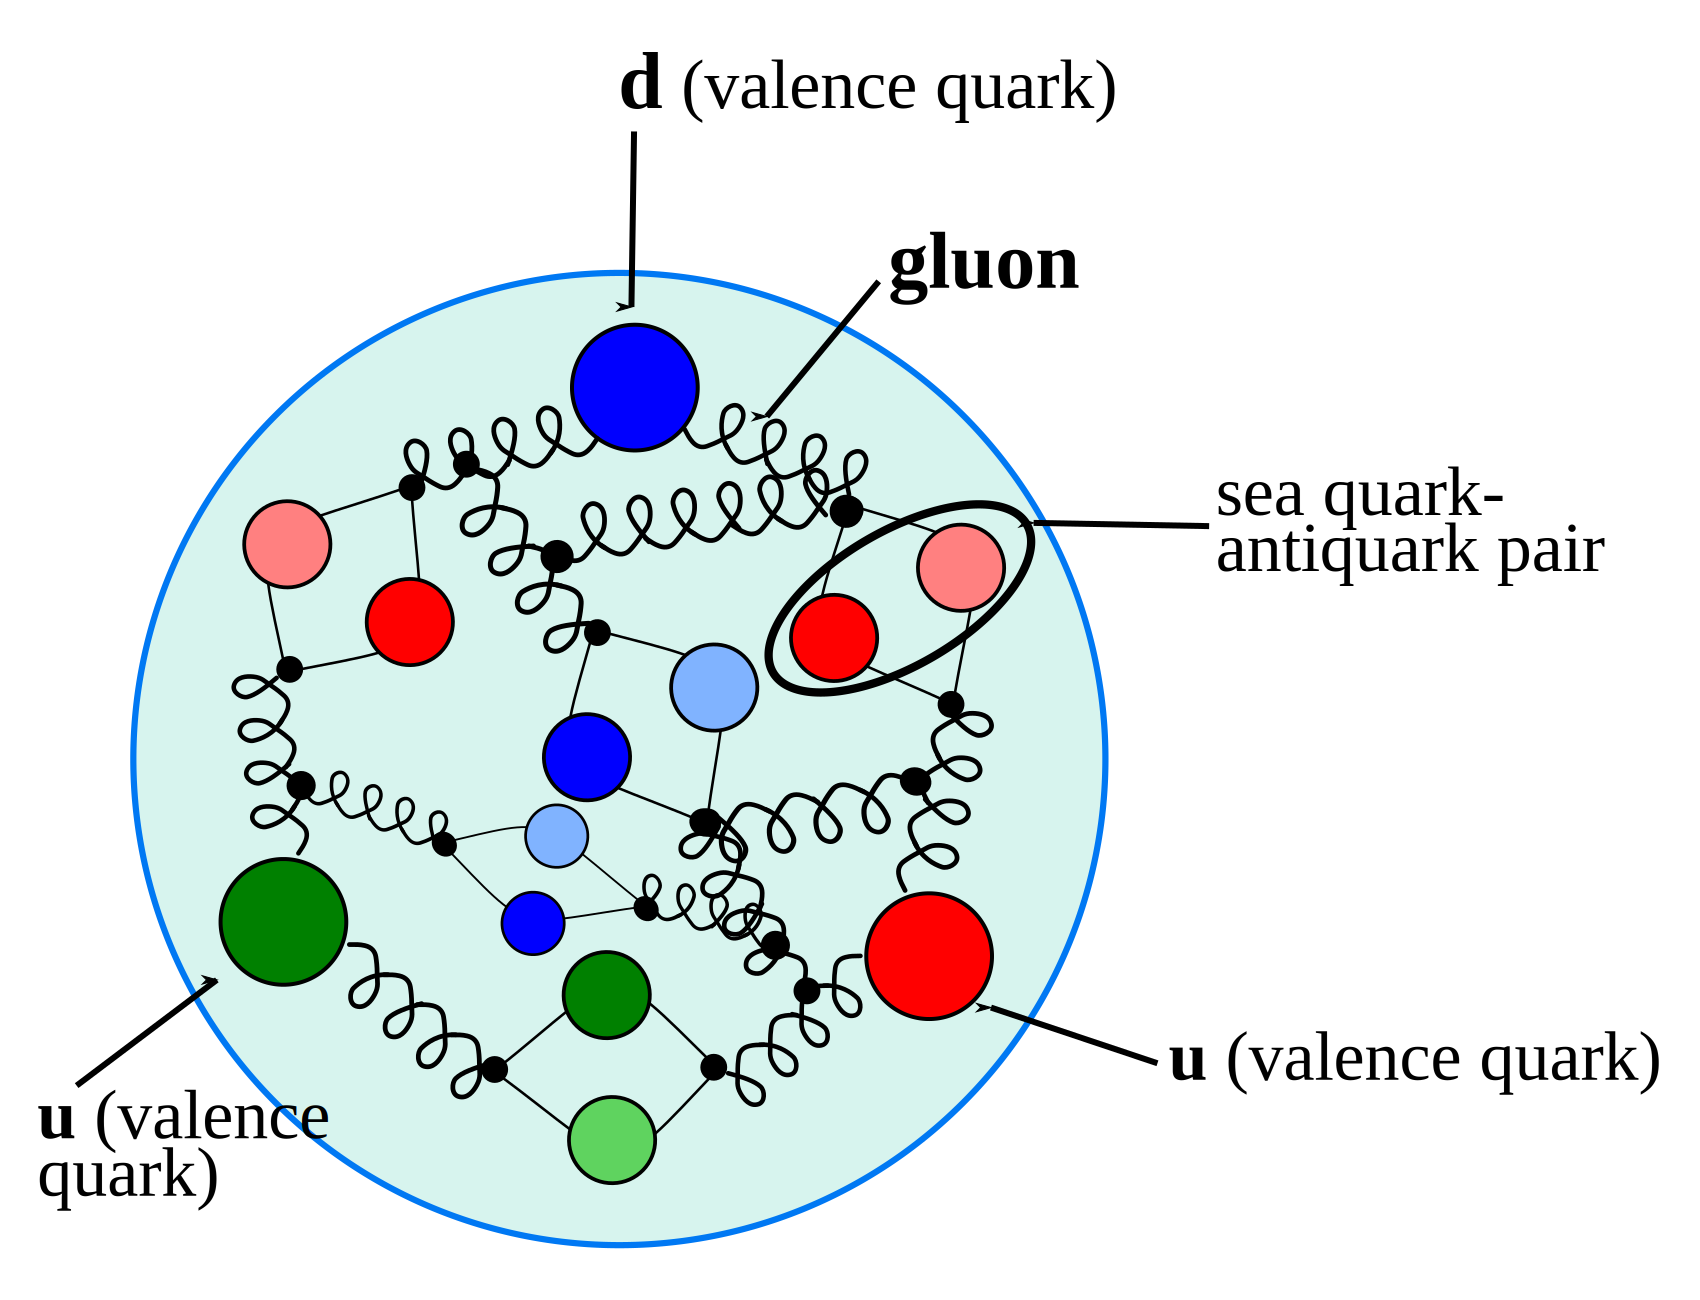
\includegraphics[width=0.45\textwidth]{../figs/Intro/protonStructure.png}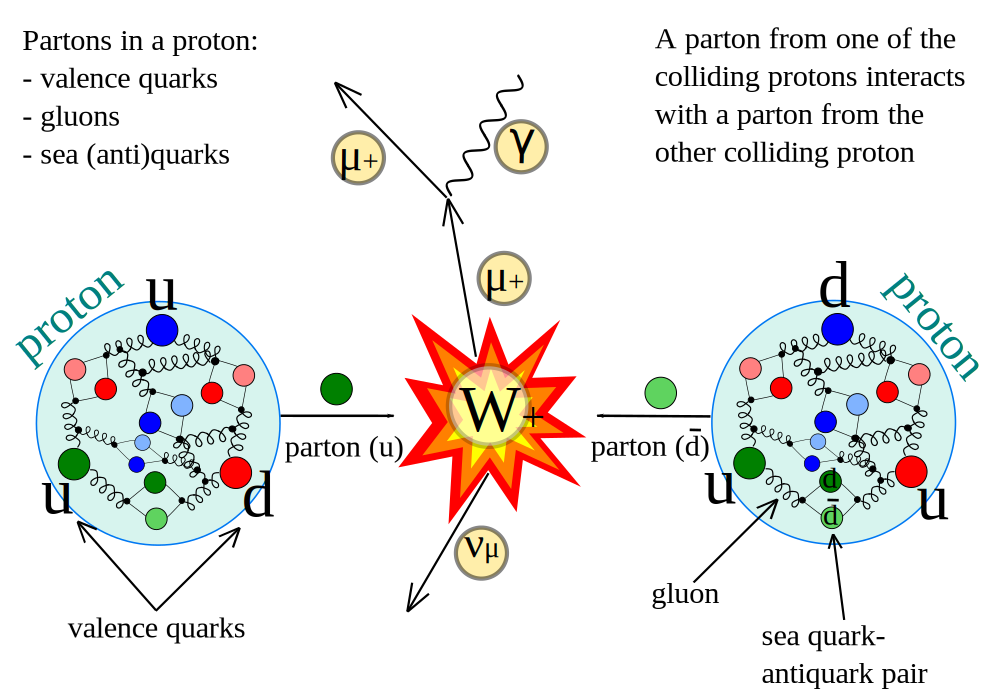
\includegraphics[width=0.45\textwidth]{../figs/Intro/ppCollision.png}}
  \end{center}
\end{figure}
\end{frame}%{Proton-Proton Collisions}


\begin{frame}\frametitle{Compact Muon Solenoid (CMS). Components}
\begin{figure}[htb]
  \begin{center}
    {\includegraphics[width=0.45\textwidth]{../figs/Exp/CMSview1.png}
     \includegraphics[width=0.45\textwidth]{../figs/Exp/CMSview.png}}
  \end{center}
\end{figure}
\end{frame}%{Compact Muon Solenoid (CMS). Components}


\begin{frame}\frametitle{Compact Muon Solenoid (CMS). Particle Reconstruction}
\begin{figure}[htb]
  \begin{center}
    {\includegraphics[width=0.98\textwidth]{../figs/Exp/CMS_Slice.png}}
  \end{center}
\end{figure}
\end{frame}%{Compact Muon Solenoid (CMS). Particle Reconstruction}

 
\begin{frame}\frametitle{Neutrino. Missing Transverse Energy}
\scriptsize
When all particles in the event are reconstructed and identified, the algorithm determines missing transverse energy $E_T^{miss}$ as 
\begin{equation}\label{eq:MET}
  E_T^{miss} = - | \sum \mathbf{P_T} |,
\end{equation}
\noindent{where the summation covers all visible particles in the event. For precise measurement of $E_T^{miss}$ it is important to capture the full energy release of all visible particles.}
\end{frame}%{Neutrino. Missing Transverse Energy}
